%%%%%%%%%%%%%%%%%%%%%%% Le TIPE !! %%%%%%%%%%%%%%%%%%%%%%%%%%%%%%%
%cc/cv de overleaf.com :s

%%%%% intro/doc info %%%%%%
\documentclass{beamer}[aspectratio = 43]
\usetheme{Frankfurt}
\usecolortheme{whale}
\title{Prédiction des décès dus au Covid19 à l'aide de machine learning.}
\subtitle{}
\author{Enzo De Carvalho}
\date{
	Numéro d'inscription : 29448\\%
	\vspace{5pt}
	2020-2021\\%
	}
\setbeamertemplate{footline}[frame number]

%%%%% packages %%%%%
\usepackage [french]{babel}
\usepackage [utf8]{inputenc}
\usepackage [T1] {fontenc}
\usepackage{xspace}
\usepackage{xurl}
\usepackage{graphicx}
\usepackage{appendixnumberbeamer}
\graphicspath{ {figures/} }


%%%%%%% Le doc %%%%%%%
\begin{document}

\begin{frame}
	\maketitle
\end{frame}

\begin{frame}
	\frametitle{Sommaire}
	\tableofcontents
\end{frame}

\section{Première approche : simple regression}
\subsection*{Principe}
\begin{frame}
	\frametitle{Principe de la démarche}
	\begin{figure}[t]
		\centering
		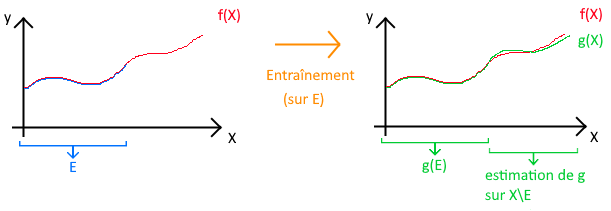
\includegraphics[scale=0.7]{super_schema}
	\end{figure}
	%\textcolor{blue}{Entraînement supervisé} :\\
	$\hookrightarrow$ le modèle $\hat{g}$ généralise les données connues $Y$ fournies.
\end{frame}

\subsection*{Regression Linéaire}
\begin{frame}
	\frametitle{Première approche : regression linéaire}
	\onslide<1->
	En utilisant \textcolor{blue}{ElasticNet} %du module \texttt{scikit-learn}.\\
	
	\vspace{0.23 cm}
	Modèle :
	\begin{figure}[h]
		\begin{minipage}{0.35\textwidth}
			$\hat{g}_{deces} (\omega,t) =\omega_{0} +  \omega_{1} t$
		\end{minipage}%
		\begin{minipage}{0.65\textwidth}
			\begin{itemize}
				\item[] $t$ les données (le temps)
				\item[] 
				$\omega = 
				\begin{pmatrix}
					\omega_{0} \\
					\omega_{1}
				\end{pmatrix}$ un paramètre à déterminer
			\end{itemize}
		\end{minipage}
	\end{figure}
	\onslide<2>
	\vspace{20pt}
	le modèle \textcolor{blue}{ElasticNet} détermine alors $\omega$.\\
	Le résultat dépend des hyperparamètres : $\alpha$ et $\rho$
	

\end{frame}

\begin{frame}
	\frametitle{Première application}
	\begin{figure}
		Prédictions entre le 2020/11/01 et 2020/12/16.
		\begin{minipage}{0.8\textwidth}
					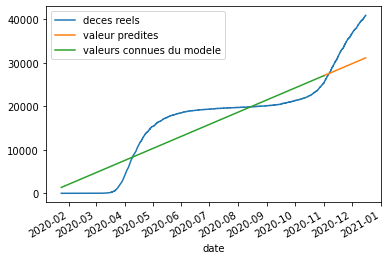
\includegraphics[scale=0.6]{EN_2020-11-01}
		\end{minipage}%
		\begin{minipage}{0.2\textwidth}
			\begin{itemize}
			\item[] $\rho = 0.9$
			\item[] $\alpha = 0.1$
			\end{itemize}
		\end{minipage}
		\caption{Résultats peu satisfaisant... (ici \texttt{l1\_ratio} est $\rho$)}
	\end{figure}
\end{frame}

\subsection*{Optimisation d'hyperparamètres}
\subsection*{Résultats avec SVR}
\begin{frame}
	\frametitle{SVR ; Premier résultat}
	Modèle \textcolor{blue}{SVR}% du module \texttt{scikit-learn}.\\
	\\
	Hyperparamètres :
	\begin{itemize}
		\item[]$C$ le paramètre de régularisation
		\item[]$\epsilon$ la taille du tube de \og non-pénalité \fg
		\item[]$\gamma$ paramètre du noyeau (\texttt{rbf} ici)
	\end{itemize}
	\onslide<2>
	\begin{figure}[h]
		\centering
		\begin{minipage}{0.5\textwidth}
			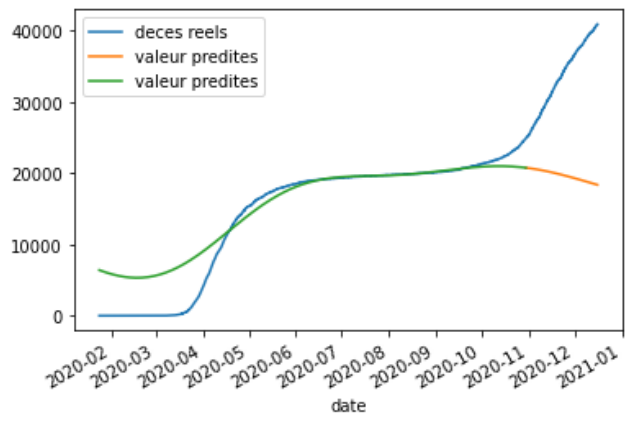
\includegraphics[scale=0.4]{svr100_}
		\end{minipage}%
		\begin{minipage}{0.5\textwidth}
			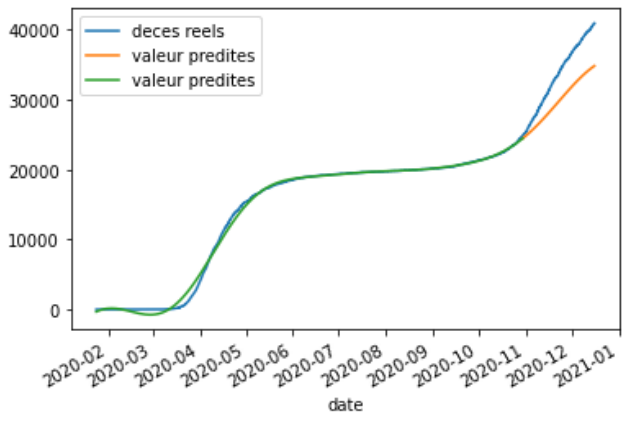
\includegraphics[scale=0.4]{svr100000_}
		\end{minipage}
		\caption{\textcolor{blue}{SVR} avec $C=100$, puis $C=100000$}
	\end{figure}
%	\begin{figure}[h]
%		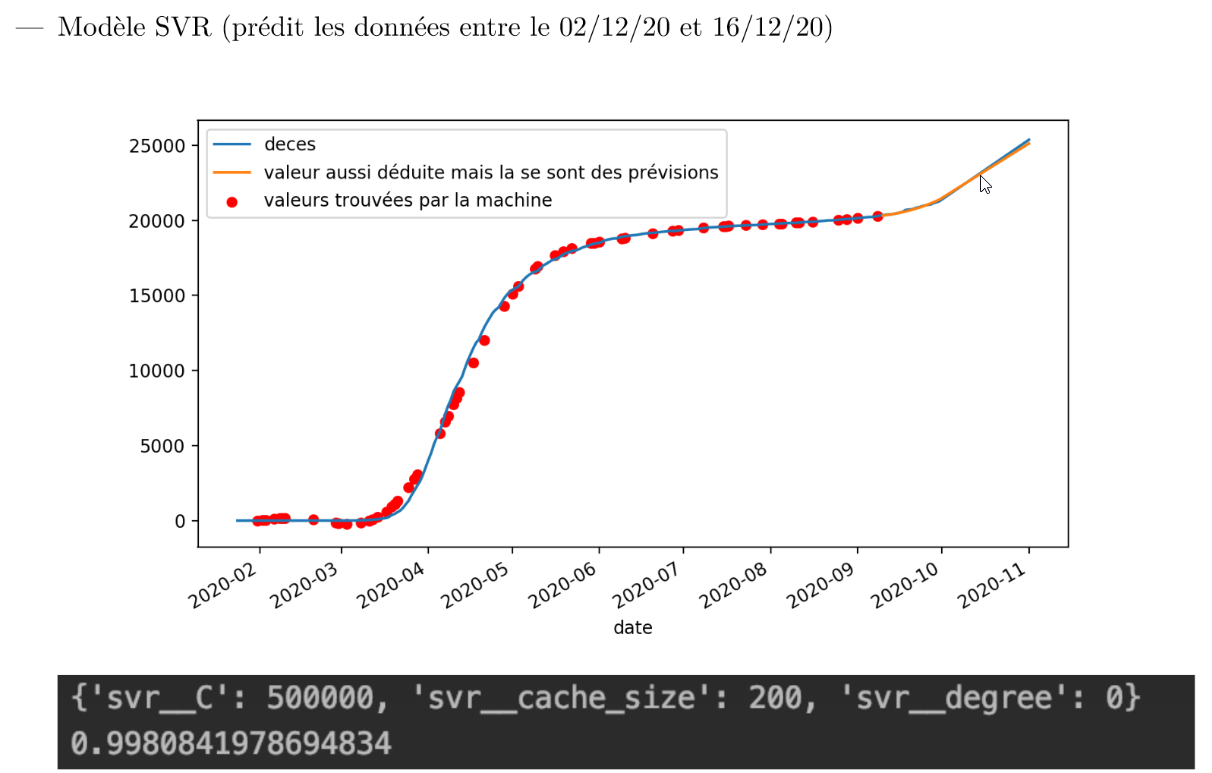
\includegraphics[scale=0.2]{SVR_premierdecoup}
%		\centering
%		\caption{Premier résultat avec SVR avec une "mauvaise stratégie d'entraînement"}
%	\end{figure}
\end{frame}

\subsubsection*{Cross-validation}
\begin{frame}
	\frametitle{Validation croisée}
	Pour une combinaison d'hyperparamètre :
	\begin{figure}[h]
		\centering
		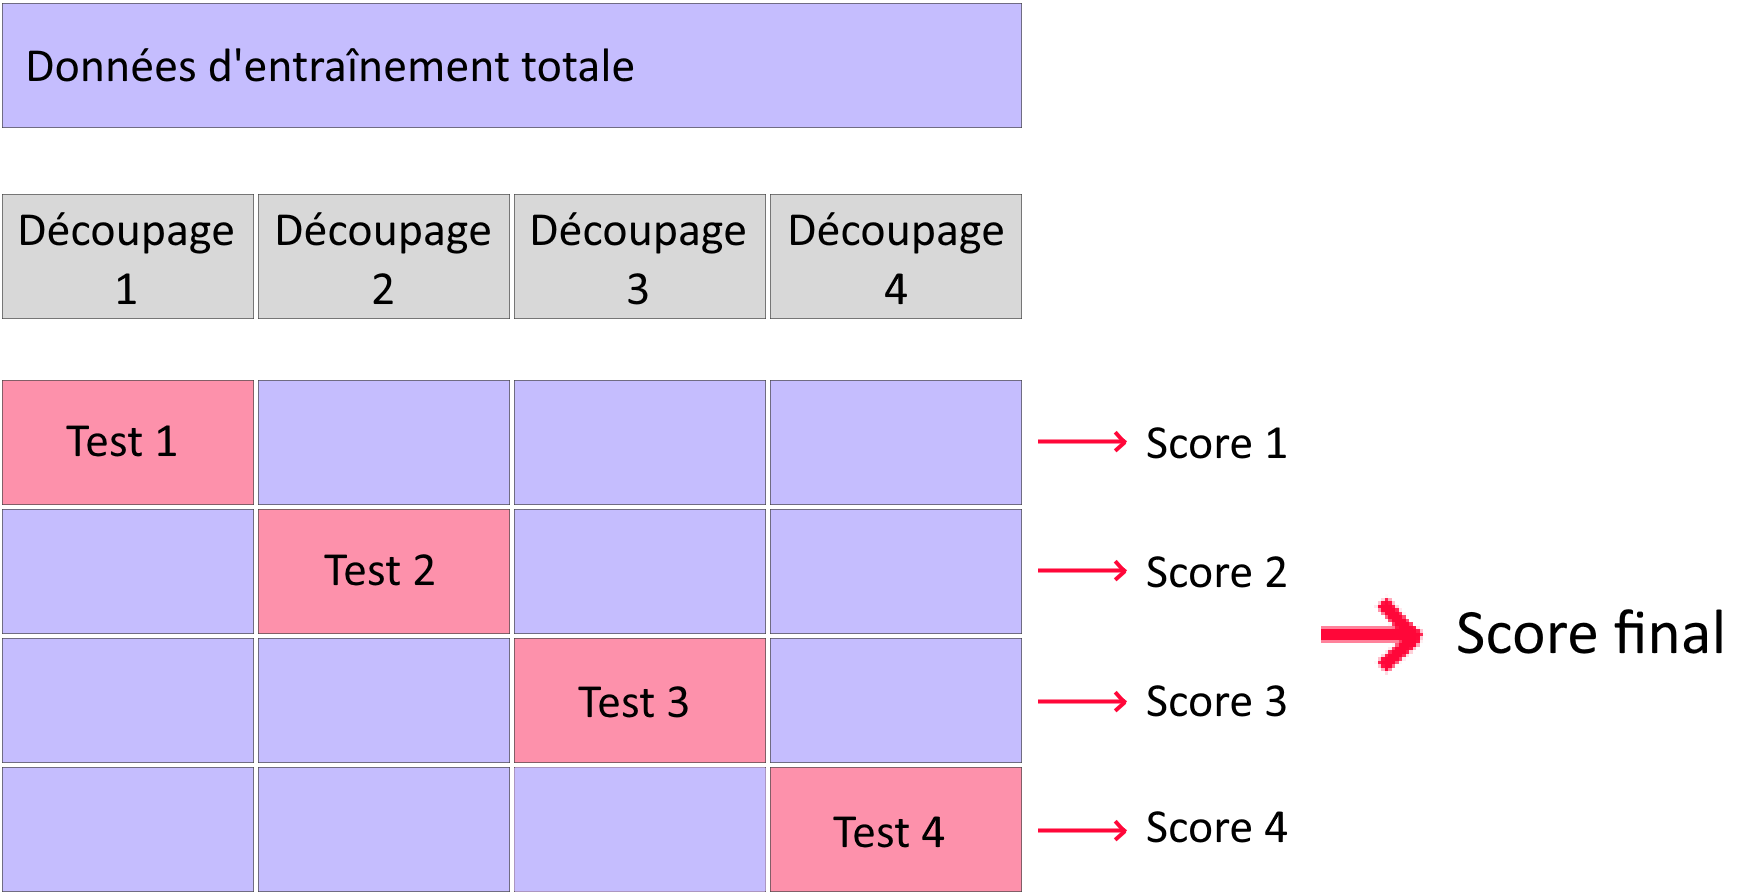
\includegraphics[scale=0.25]{VC}
	\end{figure}
\end{frame}

\begin{frame}
	\frametitle{Stratégie pour la Validation croisée}
		\begin{figure}[h]
			\centering
			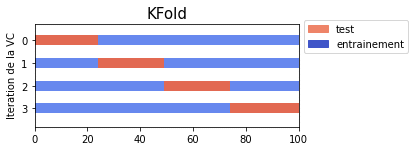
\includegraphics[scale=0.7]{kfold_}
			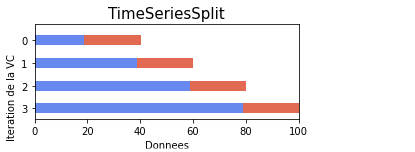
\includegraphics[scale=0.7]{tscv_}
		\end{figure}
\end{frame}

\begin{frame}
	\frametitle{Application avec SVR}
		\texttt{params = \{'svr\_\_C' : [10**i for i in range(1,8)]\}}\\
	\begin{figure}[h]
		\centering
		\begin{minipage}{0.5\textwidth}
			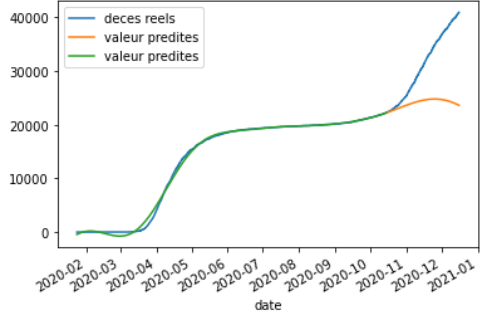
\includegraphics[scale=0.42]{SVR_avant_pt_dinflexion_}
			\centering
			\tiny{\texttt{\{'svr\_\_C' : 100000\}}}
		\end{minipage}%
		\begin{minipage}{0.5\textwidth}
			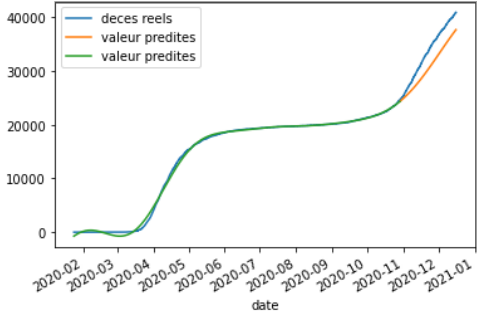
\includegraphics[scale=0.42]{SVR_apres_pt_dinflexion_}
			\centering
			\tiny{\texttt{\{'svr\_\_C' : 1000000\}}}
		\end{minipage}
	\caption{à partir du 2020/10/15, puis du 2020/11/01}
	\end{figure}
	$\Rightarrow$ \'Echec de géneralisation.
\end{frame}

\begin{frame}
	\frametitle{Prophet}
	Approche avec le modèle \textcolor{blue}{Prophet} de 
Facebook
	\begin{itemize}
		\item[]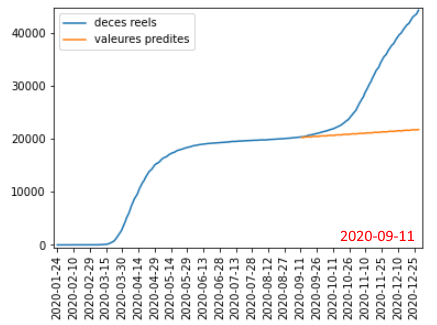
\includegraphics[scale=0.4]{prophet_bpt}
		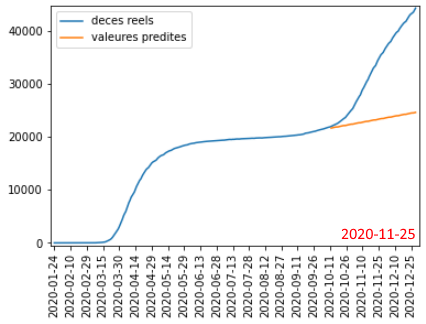
\includegraphics[scale=0.4]{prophet_mpt}
		\item[]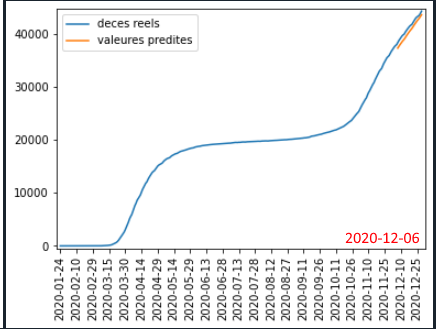
\includegraphics[scale=0.4]{prophet_ppt}
	\end{itemize}
\end{frame}

\section{Approche multivariées}
\subsection*{Multiregresseur : 'RegressorChain'}
\begin{frame}
	\frametitle{RegressorChain SVR}
	Approche multivarié avec \textcolor{blue}{RegressorChain}\\
	%\tiny{(description de scikit : \url{https://scikit-learn.org/stable/modules/generated/sklearn.multioutput.RegressorChain.html########sklearn.multioutput.RegressorChain})}\\
	%\normalsize{\textit{"Each model makes a prediction in the order specified by the chain using all of the available features provided to the model plus the predictions of models that are earlier in the chain."}}
	\texttt{params = \{\\'svr\_\_C' : [10**i for i in range(1,8)],\\ 
	'svr\_\_epsilon': [0.1,0.01,0.001]\}}\\
	\begin{figure}[h]
		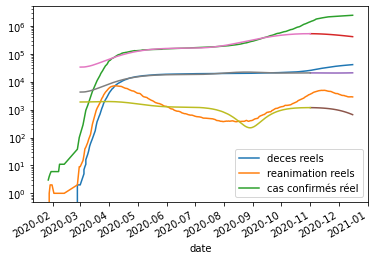
\includegraphics[scale=0.5]{mr_c10000_eps0001}
		\caption{ \textcolor{blue}{RegressorChain} avec $C = 10000$ et $\epsilon = 0.001$}
	\end{figure}
\end{frame}

\subsection*{Réseau neuronal}
\begin{frame}
	\frametitle{Réseau neuronal}
	Approche avec un \textcolor{blue}{réseau de neurone}
	\begin{figure}[t]
		\centering
		\begin{minipage}{0.5\textwidth}
			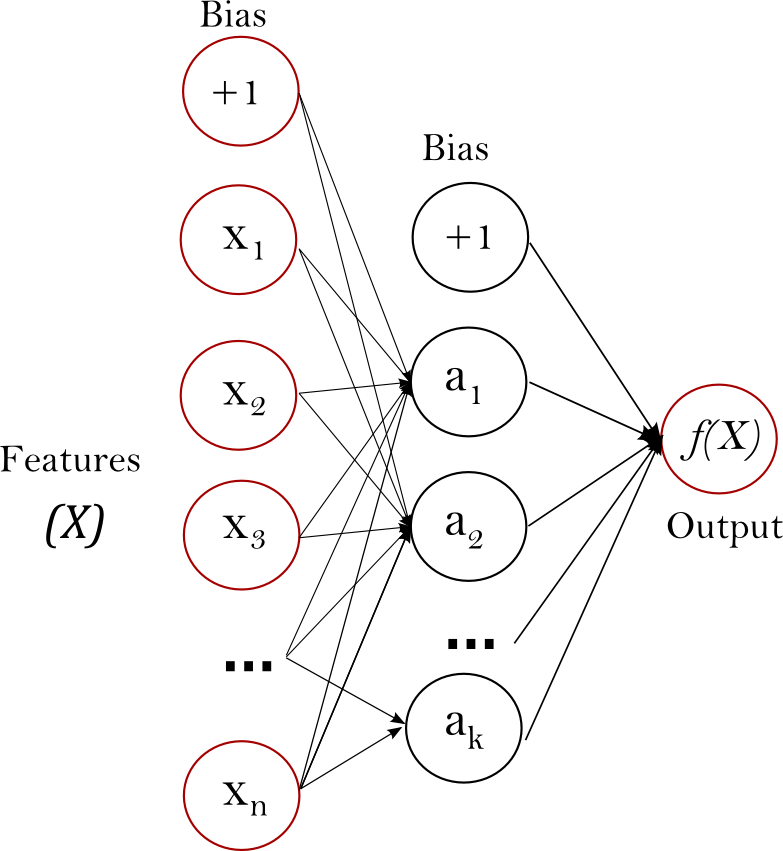
\includegraphics[scale=0.2]{nn_sk}
		\end{minipage}
		%\begin{minipage}{0.3\textwidth}
			%\tiny{Basé sur le fonctionnement du cerveau. Donne un jeu de donné successivement interprétées par un jeu de hidden layers. Un hidden layer est un jeu de neurones chacun interprétant et transformant les objets donnés pour décrypter le jeu de donnés précédents. À la fin on aboutit au résultat trouvé par la machine. Le but de l'entrainement ici est l'ajustement de chaque hidden layer et de ces neurones pour tomber sur des prédictions les plus proches possible de la réalité. $Maxiter$ est alors le nombre de fois que le modèle va s'entrainer au maximum si il n’a pas réussi à aboutir à un résultat satisfaisant la tolérance tol donnée.}
		%\end{minipage}
	%\\
	%\alert{N.B trop verbeux !}
	\end{figure}
\end{frame}

\begin{frame}
	\frametitle{Application avec réseau neuronal}
	\begin{figure}[h]
		\centering
		\begin{minipage}{0.5\textwidth}
			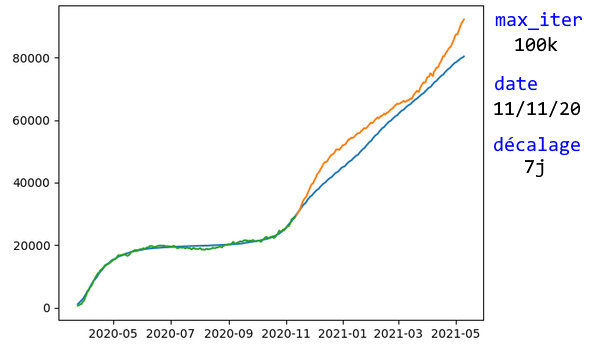
\includegraphics[scale=0.42]{NN_1_}
			\centering
		\end{minipage}%
		\begin{minipage}{0.5\textwidth}
			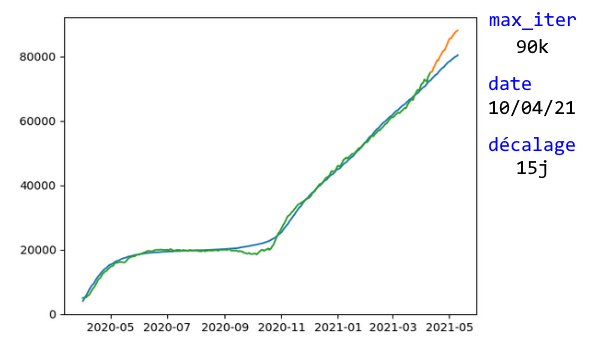
\includegraphics[scale=0.42]{NN_2_}
			\centering
		\end{minipage}
	\end{figure}
	\begin{figure}
		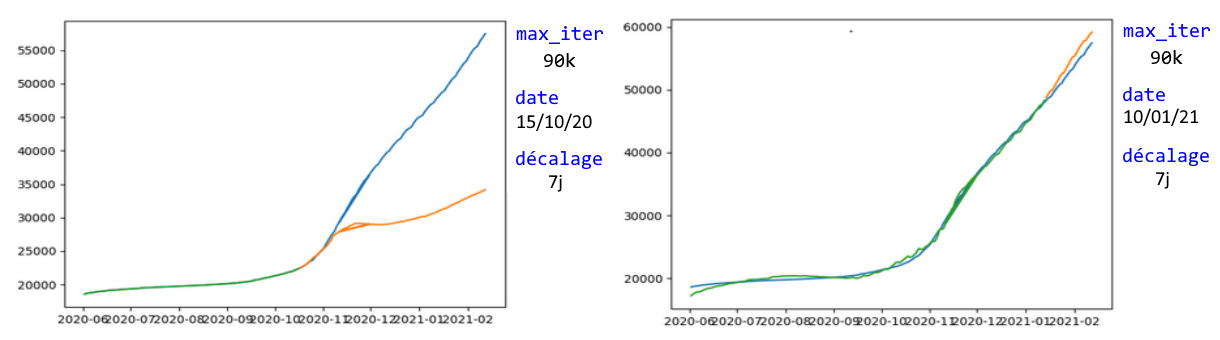
\includegraphics[scale=0.4]{NN_3_}
	\end{figure}
\end{frame}

\begin{frame}
	\frametitle{Application avec réseau neuronal}
	taux de corrélation entre\\ \texttt{total\_cas\_confirmes} et \texttt{total\_deces\_hopital} : \texttt{0.977939} 
	\begin{figure}
		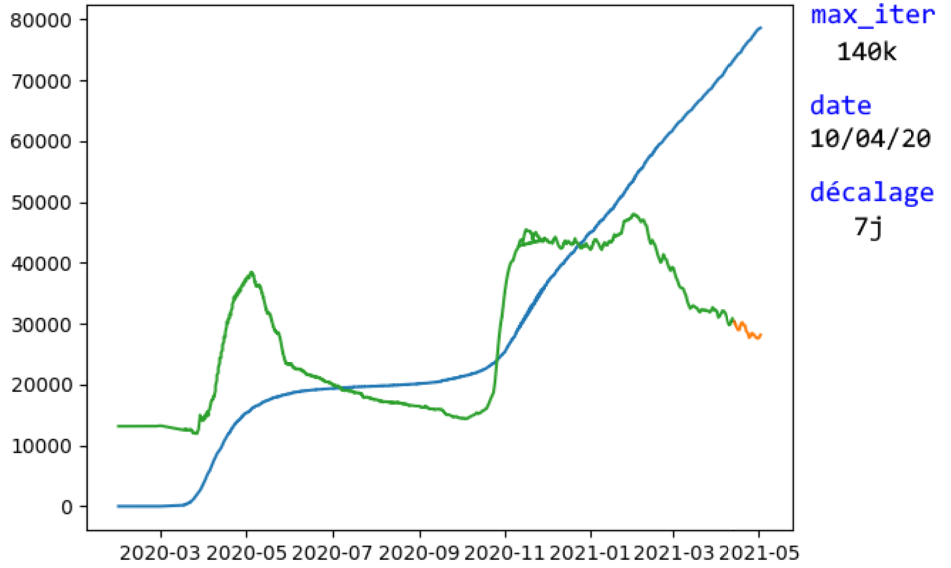
\includegraphics[scale=0.4]{NN_up_}
	\end{figure}
	$\Rightarrow$ échec du modèle sans la courbe des cas confirmés
\end{frame}

\begin{frame}
	\frametitle{Conclusion}
$\Rightarrow$ Résultats peu convaincants.
\end{frame}

%%%%%%% La fin %%%%%%%%
\appendix
%\begin{frame}
%	\frametitle{Notes}
%	\alert{N.B les diapos sont trop verbeux; il faut %encore un effort de concision, ou alors elles doivent %être expliquées à l'oral}\\
%	\alert{N.B sourcer les images}
%\end{frame}

\begin{frame}
	\frametitle{fonction d'objectif d'ElasticNet}
	\textcolor{blue}{ElasticNet} cherche $\omega$ tel que :
	\begin{figure}[h]
		$\underset{\omega}{\mathrm{min}} \; \frac{1}{2n_{deces}}||\hat{g}_{deces} (\omega,t) - f(t)||^{2}_{2} + \alpha \rho |\omega| + \frac{\alpha (1-\rho)}{2}||\omega||^{2}_{2}$
		\\
	\end{figure}
	\begin{itemize}
		\item[]$\alpha$ et $\rho$ les hyperparamètres définissant le modèle,\\
		\item[]$f$ la courbe réelle des décès.
	\end{itemize}
\end{frame}

\begin{frame}
	\frametitle{Détails sur la regression linéaire}
	\centering
	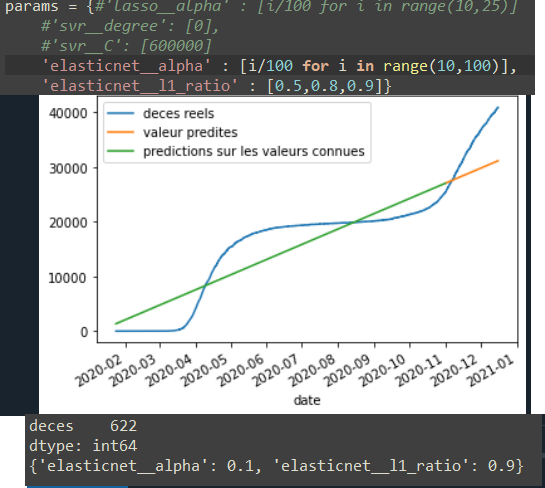
\includegraphics[scale=0.4]{EN_old}
\end{frame}

\begin{frame}
	\frametitle{Détails sur la regression multivarié}
	\centering
	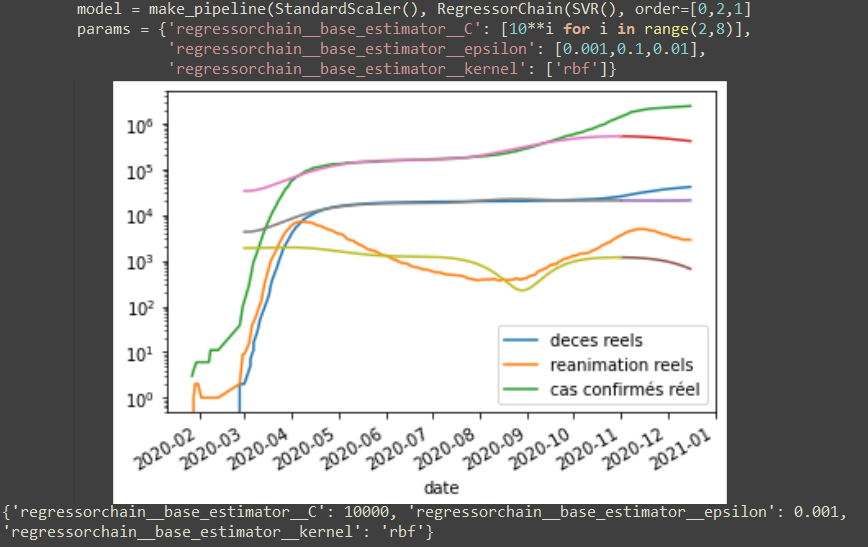
\includegraphics[scale=0.5]{Multi_regresseur}
\end{frame}

\end{document}
